\subsection{De la présence à l'apprentissage : incarnation et agence sociale}
\label{subsec:incarnation_agence_sociale}

La chaîne causale proposée par la théorie de l'agence sociale comporte quatre maillons : les indices sociaux (voix, visage, gestes) activent la présence sociale, qui génère la perception d'un partenariat, laquelle augmente l'effort de traitement et améliore l'apprentissage en profondeur \citep{moreno2001-th, mayer2012}. Ce modèle se distingue de la CTML (cf.~\ref{subsec:architecture_cognitive}) sur un point précis. Le gain d'apprentissage ne résulte pas d'une répartition optimale de l'information entre canaux cognitifs. Il résulte d'une motivation sociale à traiter le contenu plus en profondeur. Deux décennies de recherche confirment cette prédiction, tout en révélant que la nature des indices sociaux détermine l'ampleur du bénéfice \citep{veletsianos2014, johnsonlester2016}. Parmi ces indices, la voix constitue le signal le plus robuste.

La perception d'une voix humaine peut suffire à déclencher l'attribution d'un esprit à l'agent : l'auditeur infère des intentions, des émotions et une capacité de compréhension \citep{schroeder2016}. En contexte d'apprentissage, la voix humaine surpasse la voix synthétique sur les mesures de transfert et de compréhension, sans effet systématique sur la rétention factuelle \citep{craig2017}. Plusieurs méta-analyses confirment cette hiérarchie à travers des contextes variés \citep{davis2018, wang2023-meta}. La combinaison d'émotions positives et de caractéristiques vocales humaines renforce la motivation \citep{wang2021}. La prosodie --- variations de hauteur, de rythme et d'intensité --- contribue indépendamment de la qualité vocale \citep{ehret2021}. Les indices prosodiques pèsent davantage que les indices visuels dans la construction du sentiment de présence sociale. Une voix synthétique monotone peut annuler le bénéfice d'un visage expressif \citep{craig2019, chiou2020}. Des données récentes d'oculométrie confirment cette hiérarchie : la combinaison voix humaine et apparence formelle oriente l'attention vers le contenu plutôt que vers l'agent, tout en réduisant la charge cognitive \citep{xiao2025}. La qualité vocale produit un rendement supérieur à celui du raffinement visuel.

Si la voix constitue le signal le plus robuste, la composante visuelle produit des résultats plus incertains. La présence d'un corps ou d'un visage à l'écran contribue au sentiment de présence sociale et renforce l'implication émotionnelle \citep{sanghoon2015, alemdag2022-rc}. L'apparence de l'agent influence la perception de compétence et l'attitude envers le contenu \citep{domagk2010}. Un agent visible améliore le transfert par rapport à une narration seule \citep{mayer2012}. Cet avantage n'est cependant pas consistant. La majorité des études ne trouvent pas de différence d'apprentissage attribuable à la seule présence visuelle \citep{heidig2011, wangruiz2021}. Les agents en 2D produisent des résultats supérieurs à ceux en 3D \citep{castro-Alonso2021-qh}. Le réalisme géométrique ne détermine pas l'efficacité pédagogique. L'apparence agit sur les variables perceptuelles --- présence sociale, engagement, satisfaction --- sans améliorer de manière consistante l'apprentissage mesuré. L'affect lié à l'apparence constitue un facteur distinct : les agents dotés d'expressions émotionnelles améliorent la motivation et la rétention, ce qui suggère que l'effet ne transite pas par le réalisme mais par la résonance affective \citep{guo2015, shiban2015-fe}.

La distinction entre propriétés externes et internes des agents éclaire ce paradoxe \citep{moreno2004}. Les propriétés externes --- image et voix --- constituent la persona de l'agent. Les propriétés internes désignent les méthodes pédagogiques : feedback, guidage, modélisation. Les travaux conduits avec Herman The Bug, un personnage 2D enseignant la botanique, ont permis d'isoler ces dimensions \citep{lester1999}. La présence visuelle de l'agent n'affecte pas l'apprentissage lorsque les méthodes pédagogiques restent constantes. La voix suffit à activer la perception d'un partenaire. L'image, en l'absence de valeur pédagogique ajoutée, reste un \textit{seductive detail} --- un élément engageant mais non fonctionnel pour l'apprentissage \citep{harp1998, rey2012}. Les caractéristiques de persona --- apparence, genre, voix, expressions, mouvements --- interagissent de manière complexe et produisent des effets différenciés selon le niveau scolaire des apprenants \citep{tao2022}. L'alignement thématique entre l'apparence et le domaine enseigné introduit une nuance supplémentaire. Un agent congruent --- un astronaute pour l'astronomie, par exemple --- génère une présence sociale et un engagement supérieurs \citep{schmidt2019-et}. Cet effet ne se généralise pas à tous les types d'alignement. La manipulation de la tenue vestimentaire et du décor vidéo ne produit pas d'effet principal sur l'apprentissage \citep{decker2023-ss}. La tenue appropriée augmente la crédibilité perçue sans affecter l'expertise perçue. L'alignement thématique (domaine de connaissance) et l'alignement contextuel (tenue, décor) activent des processus distincts.

Ces distinctions s'inscrivent dans une classification plus large des agents pédagogiques. Le tableau~\ref{tab:typologie_agents} présente les quatre dimensions qui les différencient. La figure~\ref{fig:evolution_agents} illustre l'évolution technologique correspondante.

\begin{table}[ht]
\centering
\caption{Typologie des agents pédagogiques}
\label{tab:typologie_agents}
\small
\begin{tabular}{@{} l p{9.5cm} @{}}
\toprule
\textbf{Dimension} & \textbf{Catégories} \\
\midrule
Forme & Texte seul ; Voix seule ; Avatar 2D ; Avatar 3D ; Humain filmé \\
\addlinespace
Rôle pédagogique & Instructeur (transmission directe) ; Tuteur (guidage individualisé) ; Compagnon (collaboration entre pairs) ; Motivateur (soutien affectif) \\
\addlinespace
Anthropomorphisme & Faible (icône, robot stylisé) ; Moyen (avatar cartoon) ; Élevé (humanoïde réaliste) \\
\addlinespace
Technologie & Scriptée (arbre de décision) ; Basée règles (système expert) ; NLP/ML (traitement du langage naturel) ; IA générative (LLM) \\
\bottomrule
\end{tabular}
\end{table}

\begin{figure}[ht]
\centering
\begin{subfigure}[t]{0.3\textwidth}
    \vspace{0pt}
    \centering
    \includegraphics[width=\textwidth, height=4.5cm, keepaspectratio]{images/ch2/steve_johson1997.png}
    \caption{Steve \citep{lester1997}}
\end{subfigure}
\hfill
\begin{subfigure}[t]{0.3\textwidth}
    \vspace{0pt}
    \centering
    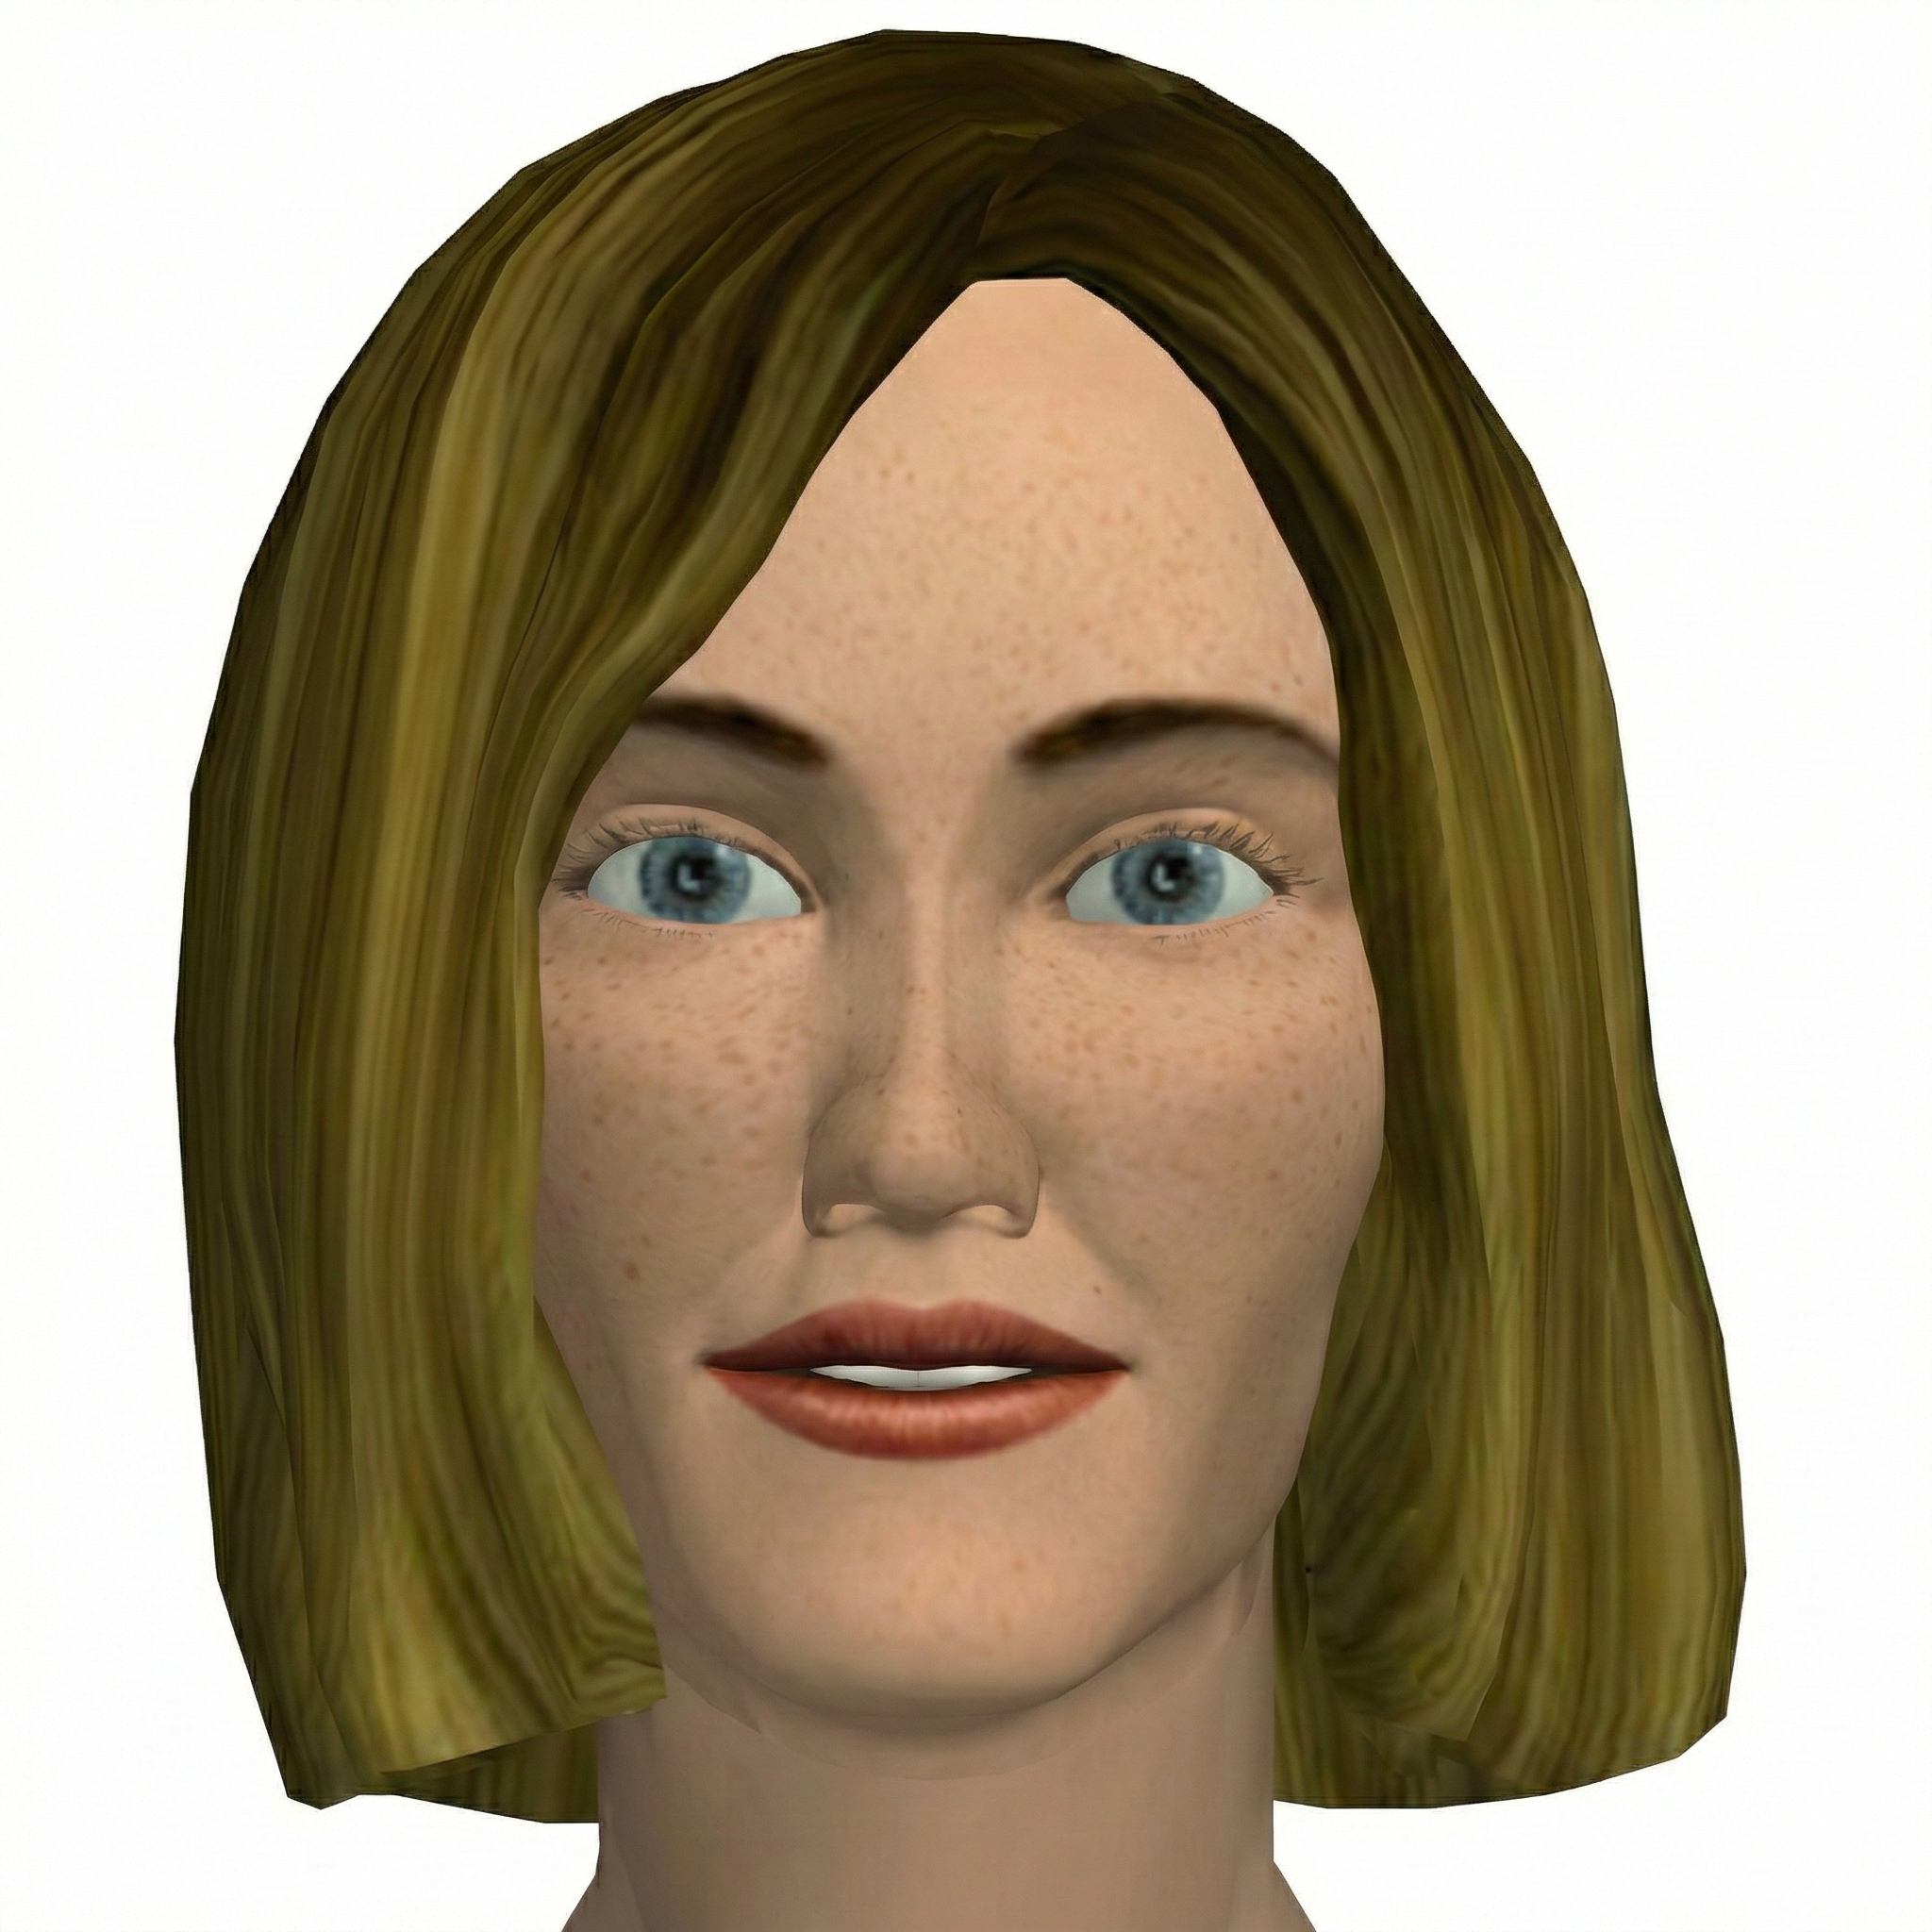
\includegraphics[width=\textwidth, height=4.5cm, keepaspectratio]{images/ch2/ochs2010.png}
    \caption{Agent expressif \citep{ochs2008}}
\end{subfigure}
\hfill
\begin{subfigure}[t]{0.3\textwidth}
    \vspace{0pt}
    \centering
    \includegraphics[width=\textwidth, height=4.5cm, keepaspectratio]{images/ch2/torre2019.png}
    \caption{Agent multimodal \citep{torre2019}}
\end{subfigure}
\caption{Évolution des agents pédagogiques sur trois décennies. De Steve (1997), premier agent pédagogique animé capable de gestes et d'expressions, aux agents expressifs modélisant des états émotionnels (2008), jusqu'aux systèmes contemporains intégrant expression multimodale et confiance (2019).}
\label{fig:evolution_agents}
\end{figure}

La distinction entre présence visuelle et comportement visuel éclaire les résultats précédents. La présence d'un corps à l'écran ne contribue pas de manière consistante à l'apprentissage, mais les comportements visuels spécifiques --- gestes, expressions, regard --- modulent la cognition par des mécanismes distincts. Les gestes déictiques --- pointer vers un élément pertinent --- dirigent l'attention vers l'information clé et améliorent l'apprentissage procédural \citep{davis2018, baylor2009}. Leur efficacité repose sur un mécanisme attentionnel, non social : ils orientent le regard et réduisent la recherche visuelle. Les expressions faciales agissent sur un registre différent. Elles favorisent l'adhésion aux messages et le changement d'attitude plutôt que l'acquisition de connaissances factuelles \citep{baylor2009}. Les gestes non liés au contenu améliorent néanmoins la rétention et le transfert, tout en augmentant le caractère humain perçu de l'agent, sans surcharge cognitive \citep{schneider2022}. Le regard direct constitue une exception. Le contact visuel augmente le temps de fixation sur l'agent, au détriment du contenu \citep{wilson2018, wang2017}. L'apprenant consacre des ressources cognitives au traitement du regard plutôt qu'au matériel pédagogique. Cet effet pourrait résulter d'un inconfort social ou d'une interférence attentionnelle non spécifique au regard.

Plusieurs méta-analyses permettent de hiérarchiser ces résultats. L'expressivité émotionnelle améliore davantage le transfert que la rétention \citep{wang2023-meta}. Cette asymétrie indique que les indices sociaux agissent sur le traitement profond --- réorganisation, application --- plutôt que sur l'encodage superficiel. La combinaison d'un design visuel et d'un rôle pédagogique défini produit des effets plus marqués que chaque dimension isolée \citep{marthasantoso2018}. L'apparence seule ne suffit pas. L'efficacité requiert une articulation entre persona et méthode pédagogique. Des résultats convergents émergent de revues systématiques récentes : la technologie sous-jacente et le type d'interaction comptent davantage que le degré de réalisme visuel \citep{dai2022-bx}.

Le profil motivationnel des agents présente cependant des limites. Les agents améliorent l'auto-efficacité et l'intérêt, mais n'ont pas d'effet détectable sur la motivation intrinsèque ni sur l'engagement \citep{gladstone2025}. Cette absence d'effet sur la motivation intrinsèque peut refléter plusieurs facteurs : une durée d'exposition insuffisante dans les protocoles expérimentaux, une mesure inadaptée au contexte technologique, ou un mécanisme distinct de ceux décrits par la SDT (cf.~\ref{subsec:sdt_cet}). La variabilité des résultats entre études indique que les bénéfices ne sont pas uniformes. Plusieurs modérateurs expliquent cette hétérogénéité. Les effets sont plus marqués chez les apprenants de 10--14 ans et chez les novices \citep{johnsonlester2016, zhang2024}. Cette tranche d'âge correspond au public cible de la thèse. Les disciplines STIM produisent des effets plus robustes que les sciences humaines \citep{alfaro2020}. L'enseignement de l'histoire, objet de cette recherche, se situe dans un domaine où les preuves sont moins solides. La stratégie pédagogique produit davantage d'effets que l'apparence. Les approches qui sollicitent activement l'apprenant --- questionnement divergent, scaffolding métacognitif, compétition ludique --- génèrent des gains d'apprentissage que le raffinement visuel de l'agent ne produit pas \citep{zhang2024}.

Ces résultats se heurtent à un plafond structurel propre aux agents classiques. Les agents scriptés fonctionnent à partir de réponses prédéfinies, sélectionnées dans un arbre de décision. Cette rigidité érode la présence sociale au fil de l'interaction \citep{schroeder2025}. L'apprenant finit par percevoir l'absence de contingence : l'agent ne répond pas de manière adaptée à ce qui a été dit. La co-construction au sens du cadre ICAP (cf.~\ref{subsec:icap}) suppose que chaque contribution s'appuie sur la précédente. Les systèmes scriptés ne fournissent pas cette adaptation sémantique en temps réel. À cette limite technologique s'ajoute un constat perceptuel. Les résultats précédents indiquent que les agents 2D tendent à produire de meilleurs résultats que les agents 3D et que le réalisme visuel ne semble pas déterminer à lui seul l'efficacité pédagogique. La relation entre l'apparence de l'agent et la réponse de l'apprenant ne suit pas un gradient linéaire.

